\documentclass[10pt,a4paper]{book}

\usepackage[utf8]{inputenc}
\usepackage[french]{babel}
\usepackage[T1]{fontenc}
\usepackage{amsmath}
\usepackage{amsfonts}
\usepackage{amssymb}
\usepackage{hyperref}
\usepackage{graphicx}
\usepackage{caption}
\usepackage{subcaption}
\usepackage{dirtree}
\usepackage[left=2cm,right=2cm,top=2cm,bottom=2cm]{geometry}

\title{Journal de bord}
\author{Gabin Serrurot}

\begin{document}

\maketitle

\tableofcontents

\part{Journal de bord}

\chapter{Janvier}

\begin{enumerate}
    \item \textbf{08/01/2024:}
        \begin{itemize}
            \item J'ai lu le dossier de présentation du projet
            \item J'ai essayé de créer une organisation sur Github afin d'avoir tous les codes au même endroit et afin d'éviter d'être dépend les uns des autres
        \end{itemize}
    \item \textbf{09/01/2024:}
        \begin{itemize}
            \item J'ai finalement décidé de ne pas faire une organisation, juste de faire un dossier dans mon compte Github et accorder l'accès à Yahya et Andréa afin de tout simplifier. De cette manière, je peux utiliser Github Desktop
            \item J'ai commencé le diagramme des cas d'utilisation "Aller à la recherche d’un actif dans l’entrepôt" avec le site \href{https://online.visual-paradigm.com}{visual-paradigm} : figure~\ref{recherche-actif.png1}
            \item J'ai commencé le diagramme des cas d'utilisation "Contrôler le chargement du camion" avec le site \href{https://online.visual-paradigm.com}{visual-paradigm} : figure~\ref{controle-chargement.png1}
            \item Il y aura aussi les diagrammes d'exigences et de déploiement à faire, même s'ils ne sont pas notés dans le dossier de présentation du projet
        \end{itemize}
    \item \textbf{10/01/2024:}
        \begin{itemize}
            \item J'ai d'abord perdu une bonne heure à essayer de debugger mon journal de bord, l'inclusion d'images ne fonctionnait pas alors qu'il manquait juste "usepackage{graphicx}" pour que tout fonctionne.
            \item J'ai repris les diagrammes que j'ai fais la veille avec M. Hacquard : figures~\ref{recherche_actif.png2} et~\ref{controle_chargement.png2} 
        \end{itemize}
    \item \textbf{11/01/2024:}
        \begin{itemize}
            \item Je me suis lancé dans les diagrammes de déploiement mais Pierre m'a dit que ces diagrammes sont à faire par équipe car ils représentent tout le système, pas chacun le sien
            \item J'ai donc décidé de faire la reformulation du cahier des charges
        \end{itemize}
    \item \textbf{12/01/2024:}
        \begin{itemize}
            \item J'ai vu pour la première fois un beacon avec M. Lejoncour
            \item J'ai commencé le cahier de recettes
        \end{itemize}
    \item \textbf{15/01/2024:}
        \begin{itemize}
            \item J'ai fais l'IHM de l'application (la veille mais faut pas le dire, cf image~\ref{idee_design_application1})
            \item J'ai continué le cahier de recettes
            \item J'ai aidé Andréa à installer \textbf{JMerise}
            \item "Définir le plan de numérotation des tags" devient "Donner un tableau exemple d'association entre les beacons et les actifs" dans \textbf{Planification des tâches du projet}
        \end{itemize}
    \item \textbf{16/01/2024:}
        \begin{itemize}
            \item Avec Yahya et Andréa nous avons fait le diagramme de déploiement (cf image~\ref{diagramme_deploiement}) et le diagramme d'exigences  (cf image~\ref{diagramme_exigences1})
            \item Le diagramme de déploiement convient bien mais par le diagramme d'exigences
            \item Pour l'IHM, je ne ferai probablement pas de système de connexion car ça rajouterait des contraintes trop importantes en terme de charge de travail, je me contenterai probablement plus d'un bouton de type "switch" pour basculer entre le mode de contrôle du chargement et le mode de recherche d'actif dans l'entrepôt
        \end{itemize}
    \item \textbf{17/01/2024:}
        \begin{itemize}
            \item Nous allons reprendre le diagramme d'exigences. En parlant avec M. Hacquard, nous avons fait deux diagrammes d'exigences, un pour le camion (cf image~\ref{diagramme_exigences_camion}) et un pour l'entrepôt (cf image~\ref{diagramme_exigences_entrepot})
            \item Nous avons également légèrement modifié le diagramme de déploiement (cf image~\ref{diagramme_deploiement2})
        \end{itemize}
    
    \newpage
    
    \item \textbf{18/01/2024:}
        \begin{itemize}
            \item Je vais commencer mes fiches de test car M. Hacquard a dit que les exigences en périphérie du diagramme d'exigences représentent les tests unitaires et les exigences plus hautes dans la hiérarchie du diagramme représentent les tests d'intégration
            \item J'ai réagencer le diagramme d'exigences de l'entrepôt pour améliorer la lisibilité
            \item J'ai perdu énormément de temps car \textbf{Github Desktop} a fait des siennes, il ne m'affichait plus les commits donc je ne pouvais pas faire de push sur mon Github. Je suis sorti de la salle sans que le problème soit résolu, espérons que ça ira mieux demain
        \end{itemize}
    \item \textbf{19/01/2024:}
        \begin{itemize}
            \item A priori Github Desktop fonctionne de nouveau, j'ai quand même pris du temps pour reprendre là où jen étais hier
            \item On a convenu avec M. Le Joncour que nous feront notre première revue non formelle vendredi prochain, le 26 janvier donc il faudra que nous fassions notre diapo lundi ou mardi prochain afin d'être pret en avance. Il s'agit d'une revue non formelle donc il n'y aura normalement pas de partie individuelle, il y a juste la présentation en groupe à faire. Pour cette revue nous attendons que Andréa et Yahya aient finis le modèle logique de données
            \item J'ai réalisé le cahier plan de numérotation des tags
            \item J'ai poursuivi les fiches de tests
        \end{itemize}
    \item \textbf{20/01/2024:}
        \begin{itemize}
            \item J'ai terminé (sur mon temps libre oui) les fiches de tests
        \end{itemize}
    \item \textbf{22/01/2024:}
        \begin{itemize}
            \item J'étais en CCF, je n'ai rien pu faire du tout je suis sorti 10 minutes avant la fin
        \end{itemize}
    \item \textbf{23/01/2024:}
        \begin{itemize}
            \item Nous avons d'abord décidé de ce que nous allions mettre dans nos diapos
        \end{itemize}
    \item \textbf{24/01/2024:}
        \begin{itemize}
            \item J'ai poursuivi les diapos
            \item Nous avons perdu environ 1h15 car nous avions une présentation sur la poursuite d'études au Québec
        \end{itemize}
    \item \textbf{25/01/2024:}
        \begin{itemize}
            \item J'ai poursuivi les diapos mais pendant peu de temps, j'ai terminé à la maison
            \item Nous avons passé beacoup de temps avec M. Hacquard car nous avons essayé une nouvelle alternative à notre MCD: notre tentative (image~\ref{MLD_proposition_nous}) et la proposition (image~\ref{MLD_proposition_hacquard})
        \end{itemize}
    \item \textbf{26/01/2024:}
        \begin{itemize}
            \item Nous sommes passé pour la première revue, non notée et informelle
        \end{itemize}
    \item \textbf{29/01/2024:}
        \begin{itemize}
            \item Les débuts ont été très compliqués, la connexion a été infernale et mes données mobiles également
            \item J'ai créé le projet sur \textbf{Android-studio} comme étant un \textbf{navigation drawer activity}
            \item J'ai commencé à créer le Figma
        \end{itemize}
    \item \textbf{30/01/2024:}
        \begin{itemize}
            \item J'ai fini \href{https://www.figma.com/proto/0Jh7ikCgIu2jUc2U5tIpNI/Tracking-BLE?type=design&node-id=1-2&t=LAlJHjfGajoQFf8A-0&scaling=scale-down&page-id=0%3A1&starting-point-node-id=1%3A2}{Figma} : image~\ref{figma_v1}
            \item J'ai essayé de lancer le projet sur Android studio avant de réellement commencer à coder mais je n'ai pas réussi, la première compilation a pris plus de 20 minutes sans aboutir
        \end{itemize}
    \item \textbf{31/01/2024:}
        \begin{itemize}
            \item J'ai essayé d'installer \textbf{JetBrains Toolbox} afin d'installer \textbf{Android Studio Giraffe} et non \textbf{Android studio Hérisson}, l'objectif étant de voir si la version trop récente aurait pu expliquer les problèmes de création de projet
            \item A priori la solution ne venait pas uniquement de là, j'ai créé un dossier dans mes documents et fais un lien avec github
            \item J'en ai également profité pour refaire mon architecture dossier du projet. J'ai tout mis dans mes documents avec cette architecture:
            \begin{center}
                \begin{verbatim}
                    Documents/
                        Tracking-BLE/
                            Tracking-BLE-Code/
                                Le reste
                            Tracking-BLE-documents/
                                Le reste
                \end{verbatim}
            \end{center}
        \end{itemize}
\end{enumerate}

\chapter{Février}

\begin{enumerate}
    \item \textbf{01/02/2024:}
        \begin{itemize}
            \item J'ai enfin commencé le développement
            \item J'ai essayé de mettre l'application provenant de \href{https://github.com/Gabin221/android-beacon-library-reference-kotlin}{github} sur mon téléphone afin d'avoir une balise fonctionnelle en permanance
            \item J'ai rempli la base de données avec des valeurs random pour soulager Yahya
        \end{itemize}
    \item \textbf{02/02/2024:}
        \begin{itemize}
            \item J'ai modifié les fichiers du projet de l'application afin d'avoir les noms de fichier corrects, les bons logos dans le menu et les bonnes redirections entre chaque page. Désormais, l'application ressemble visuellement à ce que je voulais
        \end{itemize}
    \item \textbf{05/02/2024:}
        \begin{itemize}
            \item J'ai ajouté un séparateur entre les éléments du menu afin d'isoler les paramètres
            \item J'ai ajouté une table \textbf{parametres} afin d'ajouter en base de données certains paramètres de l'application: 
                \begin{itemize}
                    \item major pour trier quels beacons essayer de détecter
                \end{itemize}
            \item J'ai modifié l'image du logo de l'application pour avoir le logo de l'entreprise
            \item J'ai essayé de commencer à remplir la page des paramètres mais le problème est la difficulté apparente à créer des champs de saisie ainsi que du texte à afficher
        \end{itemize}
    \item \textbf{06/02/2024:}
        \begin{itemize}
            \item J'ai essayé de commencer à remplir la page des paramètres mais le problème est la difficulté apparente à créer des champs de saisie ainsi que du texte à afficher
            \item J'ai donc essayé d'utiliser le code de \href{https://github.com/Gabin221/android-beacon-library-reference-kotlin}{l'application} afin de commencer à remplir mon application mais je me suis rendu compte que l'utilisation de ces codes allait être vraiment compliquée, par exemple le code semble appeler une classe ou un fichier \textbf{beacon} qui semble ne pas exister. M. Le Joncour ne semble pas plus comprendre que moi et nous avons galéré à comprendre ce qui se passe, en vain
        \end{itemize}
    \item \textbf{07/02/2024:}
        \begin{itemize}
            \item Je vais essayer de nouveau de comprendre comment incorporer le code de l'appli dans le miens en espérant avoir un meilleur succès que hier
        \end{itemize}
    \item \textbf{08/02/2024:}
        \begin{itemize}
            \item Je n'ai toujours pas plus réussi hier donc je vais essayer de retrouver moi-même comment détecter les beacons environnants afin de l'intégrer au mieux dans mon application
        \end{itemize}
    \item \textbf{09/02/2024:}
        \begin{itemize}
            \item Finalement M. Le Joncour a réussi à me montrer comment utiliser la recherche de beacons grâce à \href{https://altbeacon.github.io/android-beacon-library/configure.html}{ce lien} donc je vais normalement pouvoir garder mon application de base
            \item Le seul problème va être de découvrir comment écrire dedans, comment passer de 2 fichiers par page à un seul
        \end{itemize}
    \item \textbf{12/02/2024:}
        \begin{itemize}
            \item Grâce à mon application perso, je sais maintenant passer de deux fichiers à un seul donc je vais essayer finalement de remplir en premier lieu la page du camion
            \item J'ai obtenu l'application de M. Le Joncour permettant de détecter les beacons environnants: \textbf{app\_basic\_view}
            \item J'ai finalement réussi à afficher les beacons environnants dans la page camion ce qui me permet d'avoir une liste à jour en permanance
        \end{itemize}
    \item \textbf{13/02/2024:}
        \begin{itemize}
            \item Je vais essayer aujoud'hui de configurer un beacon en eddystone afin d'avoir une valeur de température
            \item Finalement ça s'annonce trop compliqué, j'ai beaucoup essayé mais M. Le Joncour m'a conseillé de faire le reste avant de regarder le eddystone
        \end{itemize}
    \item \textbf{14/02/2024:}
        \begin{itemize}
            \item Je vais essayer d'encapsuler la listeview des beacons dans un genre de frame (si ça existe) afin d'avoir quelque chose de plus agréable à regarder et à utiliser
            \item En fait il n'y a pas besoin du tout, il suffit de paramétrer les dimensions de la listeview
            \item Finalement je vais plutôt commencer à préparer le visuel de l'application maintenant que je me suis bien mis dans le XML
            \item J'ai aujourd'hui fais toute la page du camion, la seule chose qui manquera ce sera l'affichage de la température
        \end{itemize}
    \item \textbf{15/02/2024:}
        \begin{itemize}
            \item Il va maintenant falloir que je fasse la page des paramètres de l'application
            \item Il faut regarder comment afficher un \textbf{EditText}
            \item J'ai résolu ce problème, il fallait passer l'argument \textbf{android:layout\_height="match\_parent"} à \textbf{android:layout\_height="wrap\_content"}, j'étais persudadé de l'avoir fais hier mais apparement pas
            \item Il faudra que j'utilise l'expression régulière REGEX \textbf{\^~[A-Z]\{2\}[-][0-9]\{3\}[-][A-Z]\{2\}\$} SANS L'ESPACE APRES LE CIRCONFLEXE pour la saisie de la plaque d'immatriculation
        \end{itemize}
    \item \textbf{16/02/2024:}
        \begin{itemize}
            \item J'ai fais la validation du formulaire de saisie de l'immatriculation
            \item J'ai également fais pour que lorsque l'utilisateur valide sa saisie, l'application affiche le succès ou l'échec de la saisie
        \end{itemize}
\end{enumerate}

\chapter{Mars}

\begin{enumerate}
    \item \textbf{04/03/2024:}
        \begin{itemize}
            \item J'ai commencé par formatter l'affichage de la liste des couples major-minor sur la page du camion
            \item J'ai ensuite fais les éléments graphiques de la page de l'entrepôt
        \end{itemize}
    \item \textbf{05/03/2024:}
        \begin{itemize}
            \item J'ai abandonné l'idée de faire une liste dans une fenêtre modale, ça aurait été je pense une bonne idée niveau UX mais c'est trop de prise de tête pour si peu au final
            \item Je me suis beaucoup pris la tête pour modifier de nouveau la page de l'entrepôt. J'ai changé de place le bouton de validation car a priori en sélectionnant dans la liste ça effectue quand même l'action sans attendre le bouton valider ce qui est pas si mal
            \item J'ai également pris beaucoup de temps à essayer de faire l'affichage de la distance mais c'est une vraie prise de tête: soit l'application crash, soit le fait de cliquer sur un élément de la liste ne le sélectionne pas vraiment étant donné que rien ne se passe ou encore la distance s'affiche mais il faut que je sélectionne l'élément dans la liste chaque fois que je veux mettre à jour la distance étant donné qu'elle ne se met pas à jour seule
            \item Les prochaines séances vont être consacrées à la revue qui approche dans la semaine prochaine (sans doutes lundi ou mardi)
        \end{itemize}
    \item \textbf{06/03/2024:}
        \begin{itemize}
            \item J'ai commencé par créer le dossier contenant la deuxième revue ainsi que son organisation
            \item J'ai vidé la présentation commune de tout ce qui ne la concernait pas
            \item J'ai refais les schémas que nous avions pris au cahier des charges
            \item J'ai commencé mes diapos
        \end{itemize}
    \item \textbf{07/03/2024:}
        \begin{itemize}
            \item J'ai terminé mes diapos
        \end{itemize}
    \item \textbf{08/03/2024:}
        \begin{itemize}
            \item J'ai essayé de voir comment faire des requêtes SQL en Kotlin
        \end{itemize}
    \item \textbf{11/03/2024:}
        \begin{itemize}
            \item Nous avons fais nos diapos pour la partie commune
            \item J'ai essayé de terminer l'affichage de la distance
        \end{itemize}
    \item \textbf{12/03/2024:}
        \begin{itemize}
            \item Nous avons terminé nos diapos
            \item Nous sommes passé en présentation
            \item Nous sommes sortis quasiment pour la fin donc rien de plus aujdourd'hui
        \end{itemize}
    \item \textbf{13/03/2024:}
        \begin{itemize}
            \item J'ai réussi à faire que la requête HTTP me renvoie la liste complète des beacons stockés en BDD
            \item Je n'ai pas réussi à faire pour que le résultat de la requête aille dans une variable
            \item J'ai terminé la séance en faisant du PIX
        \end{itemize}
    \item \textbf{14/03/2024:}
        \begin{itemize}
            \item Je vais essayer de faire pour que le contenu de la requête puisse être stocké dans une variable
            \item J'y suis arrivé mais le problème vient de la synchronisation entre la fonction qui fait la requête et le reste. Il faudra donc que je cherche à gérer l'asynchronisation entre les différentes parties de mon code (peut-être en ajoutant un dashboard afin de lancer la requête plus tôt)
        \end{itemize}
    \item \textbf{15/03/2024:}
        \begin{itemize}
            \item Pour simplifier et gagner du temps je vais essayer de lire les beacons configurés en eddystone
        \end{itemize}
    \item \textbf{18/03/2024:}
        \begin{itemize}
            \item Je vais essayer de terminer la lecture des beacons configurés en eddystone
        \end{itemize}
    \item \textbf{19/03/2024:}
        \begin{itemize}
            \item Je vais essayer finalement de créer le datastore afin d'enregistrer certaines valeurs en local
            \item J'ai réussi à initialiser une liste avec les beacons de la base de données
        \end{itemize}
    \item \textbf{20/03/2024:}
        \begin{itemize}
            \item J'ai réussi à gérer le datastore, désormais les données sont enregistrées en local
            \item Il faudra cependant veiller à faire pour que la validation de la saisie d'une plaque d'immatriculation et que l'enregistrement en local de la plaque fonctionnent en même temps
        \end{itemize}
\end{enumerate}

\chapter{Avril}

\begin{enumerate}
    \item 
\end{enumerate}

\chapter{Mai}

\begin{enumerate}
    \item 
\end{enumerate}

\chapter{Juin}

\begin{enumerate}
    \item 
\end{enumerate}

\part{Notes pour plus tard}

\begin{itemize}
    \item Pour faire des requêtes HTTP en Kotlin, on peut utiliser "volley" de google
    \item \href{https://developer.android.com/topic/libraries/architecture/datastore?hl=fr\#kts}{https://developer.android.com/topic/libraries/architecture/datastore?hl=fr\#kts}
    \item \href{https://medium.com/androidmood/stockage-de-données-avec-jetpack-datastore-5da427bd7323}{https://medium.com/androidmood/stockage-de-données-avec-jetpack-datastore-5da427bd7323}
    \item \href{https://medium.com/@hasperong/get-current-location-with-latitude-and-longtitude-using-kotlin-2ef6c94c7b76}{https://medium.com/@hasperong/get-current-location-with-latitude-and-longtitude-using-kotlin-2ef6c94c7b76}
    \item \href{https://altbeacon.github.io/android-beacon-library/distance\_vs\_time.html}{https://altbeacon.github.io/android-beacon-library/distance\_vs\_time.html}
    \item L'URL à contacter pour recevoir la liste des major-minor est \href{https://juleshaag.fr/trackingble2024/liste\_beacons.php}{https://juleshaag.fr/trackingble2024/liste\_beacons.php}
\end{itemize}

\part{Annexes}

\begin{figure}[h!]
    \centering
    \begin{subfigure}[b]{0.45\textwidth}
        \centering
        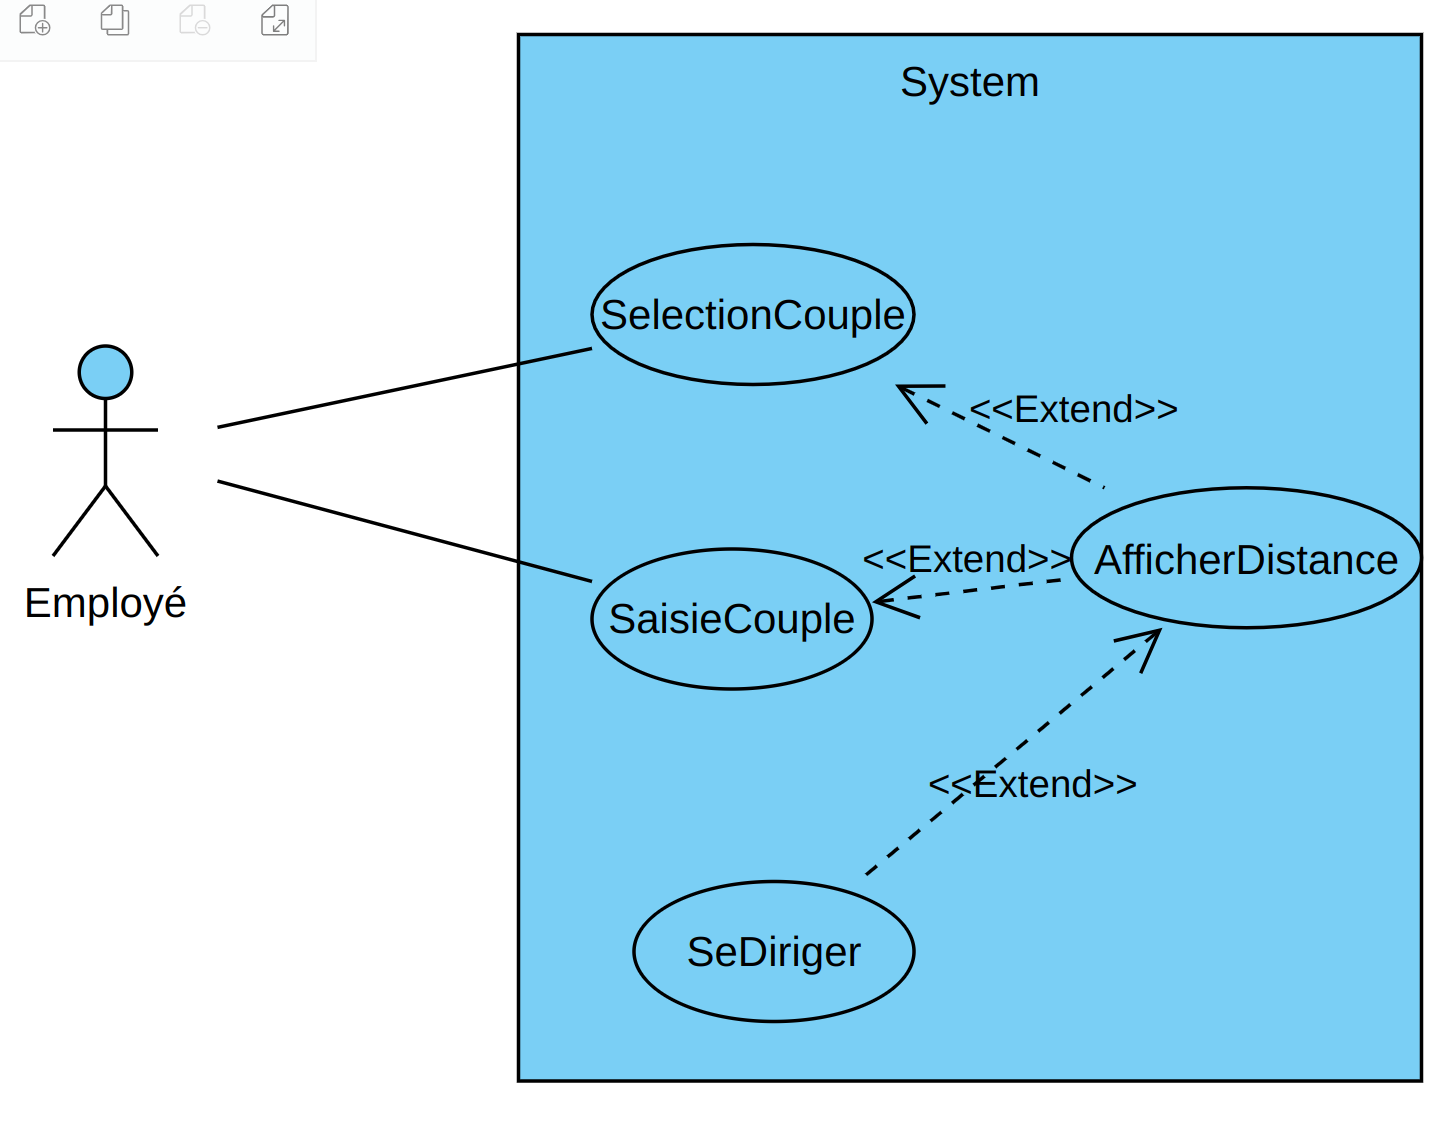
\includegraphics[scale=0.14]{Images/recherche-actif.png}
        \caption{}
        \label{recherche-actif.png1}
    \end{subfigure}
    \begin{subfigure}[b]{0.45\textwidth}
        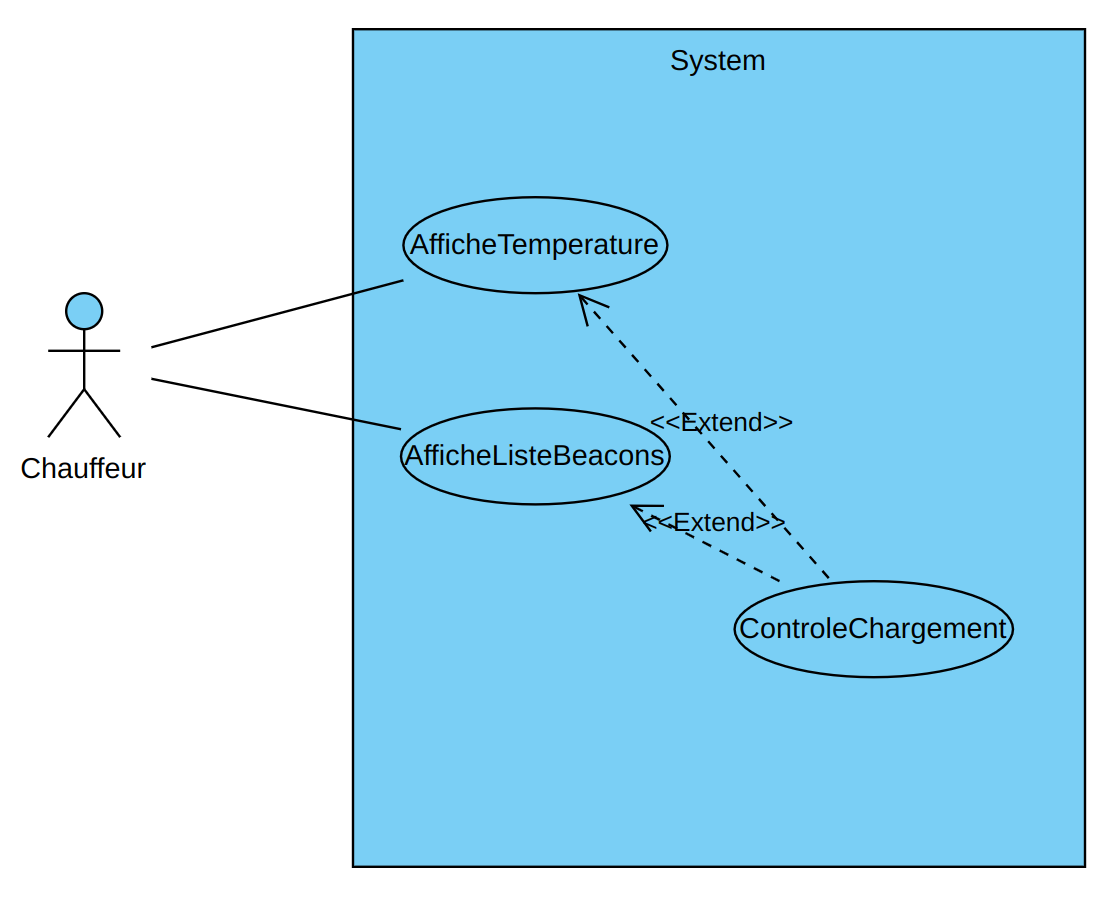
\includegraphics[scale=0.14]{Images/controle-chargement.png}
        \caption{}
        \label{controle-chargement.png1}
    \end{subfigure}
    \caption{}
\end{figure}

\begin{figure}[h!]
    \centering
    \begin{subfigure}[b]{0.45\textwidth}
        \centering
        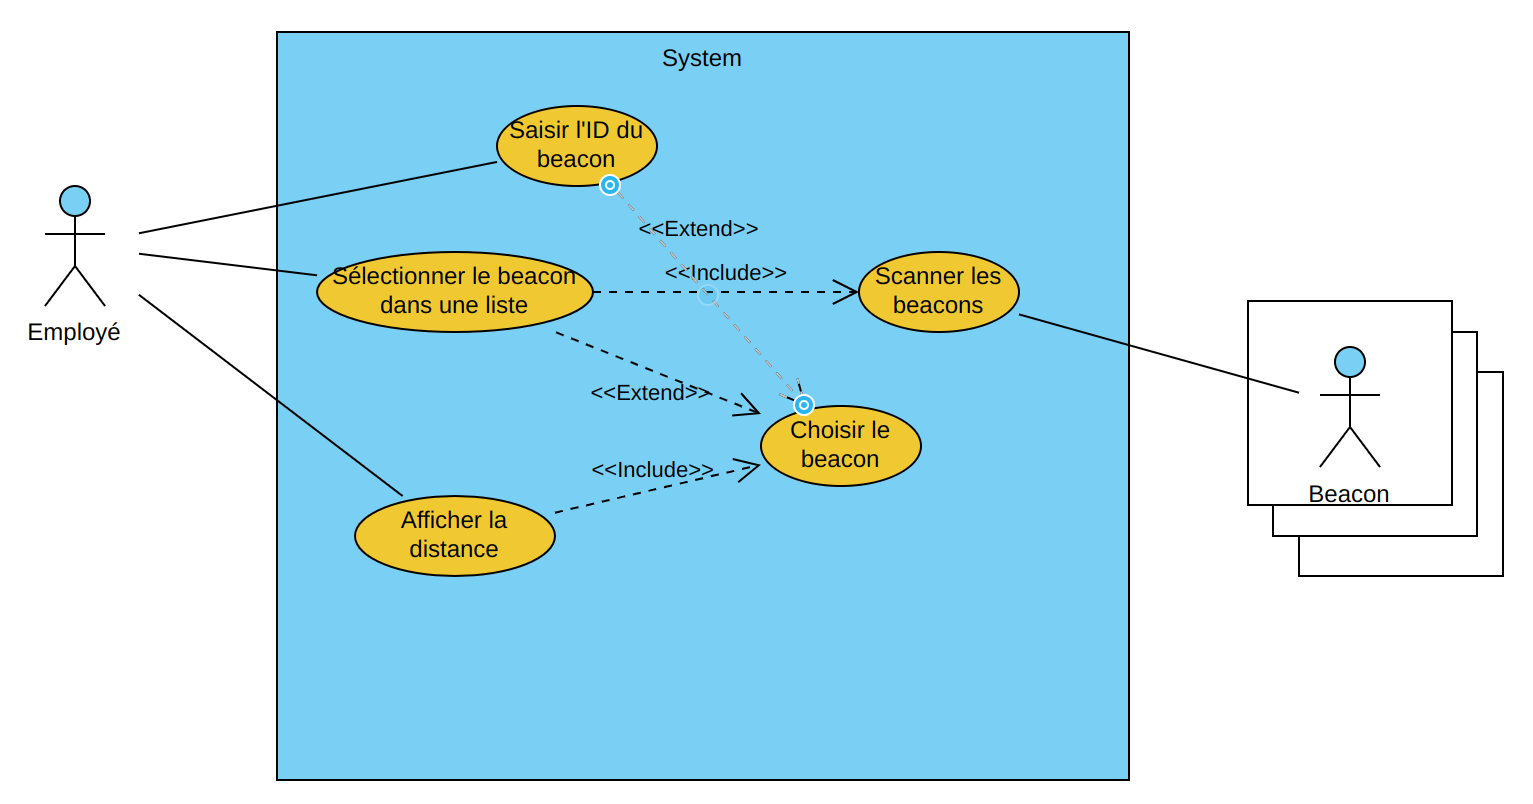
\includegraphics[scale=0.14]{Images/recherche_actif.png}
        \caption{}
        \label{recherche_actif.png2}
    \end{subfigure}
    \begin{subfigure}[b]{0.45\textwidth}
        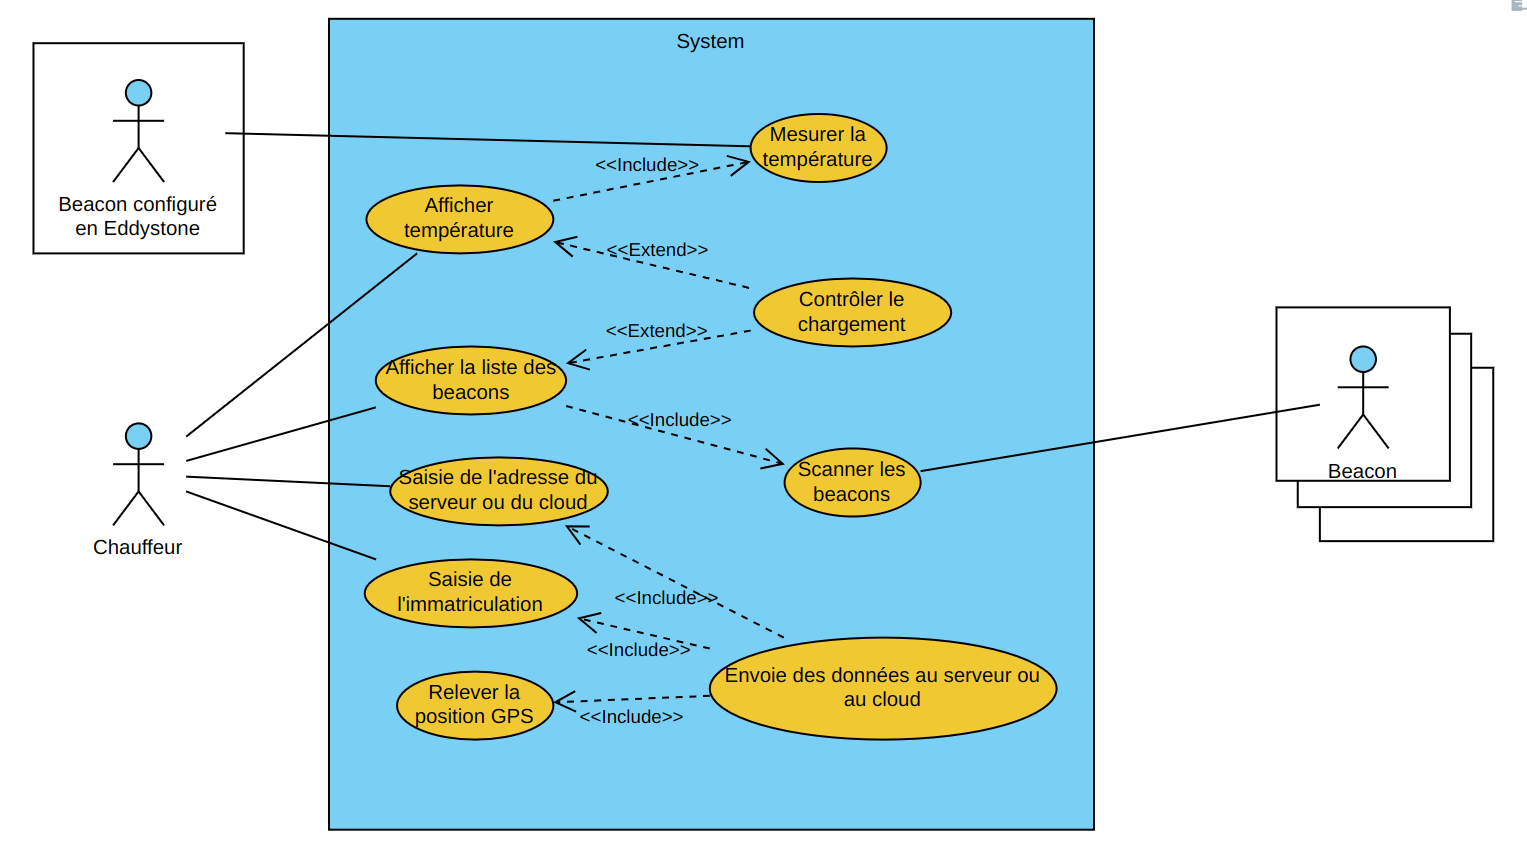
\includegraphics[scale=0.14]{Images/controle_chargement.png}
        \caption{}
        \label{controle_chargement.png2}
    \end{subfigure}
    \caption{}
\end{figure}

\begin{figure}[h!]
    \centering
    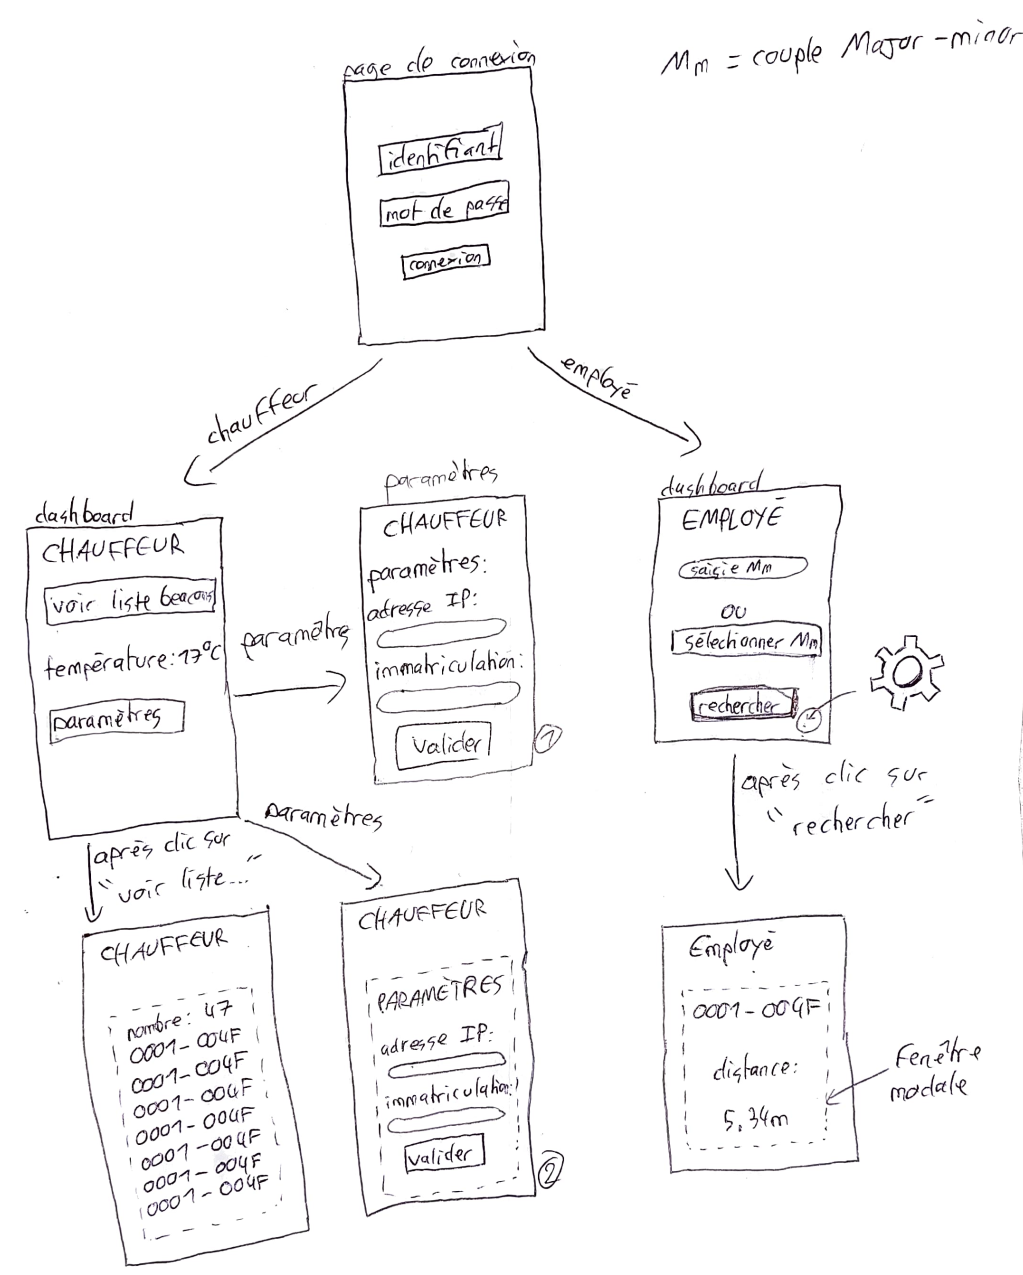
\includegraphics[scale=0.2]{Images/idee_design_application1.png}
    \caption{}
    \label{idee_design_application1}
\end{figure}

\begin{figure}[h!]
    \centering
    \begin{subfigure}[b]{0.45\textwidth}
        \centering
        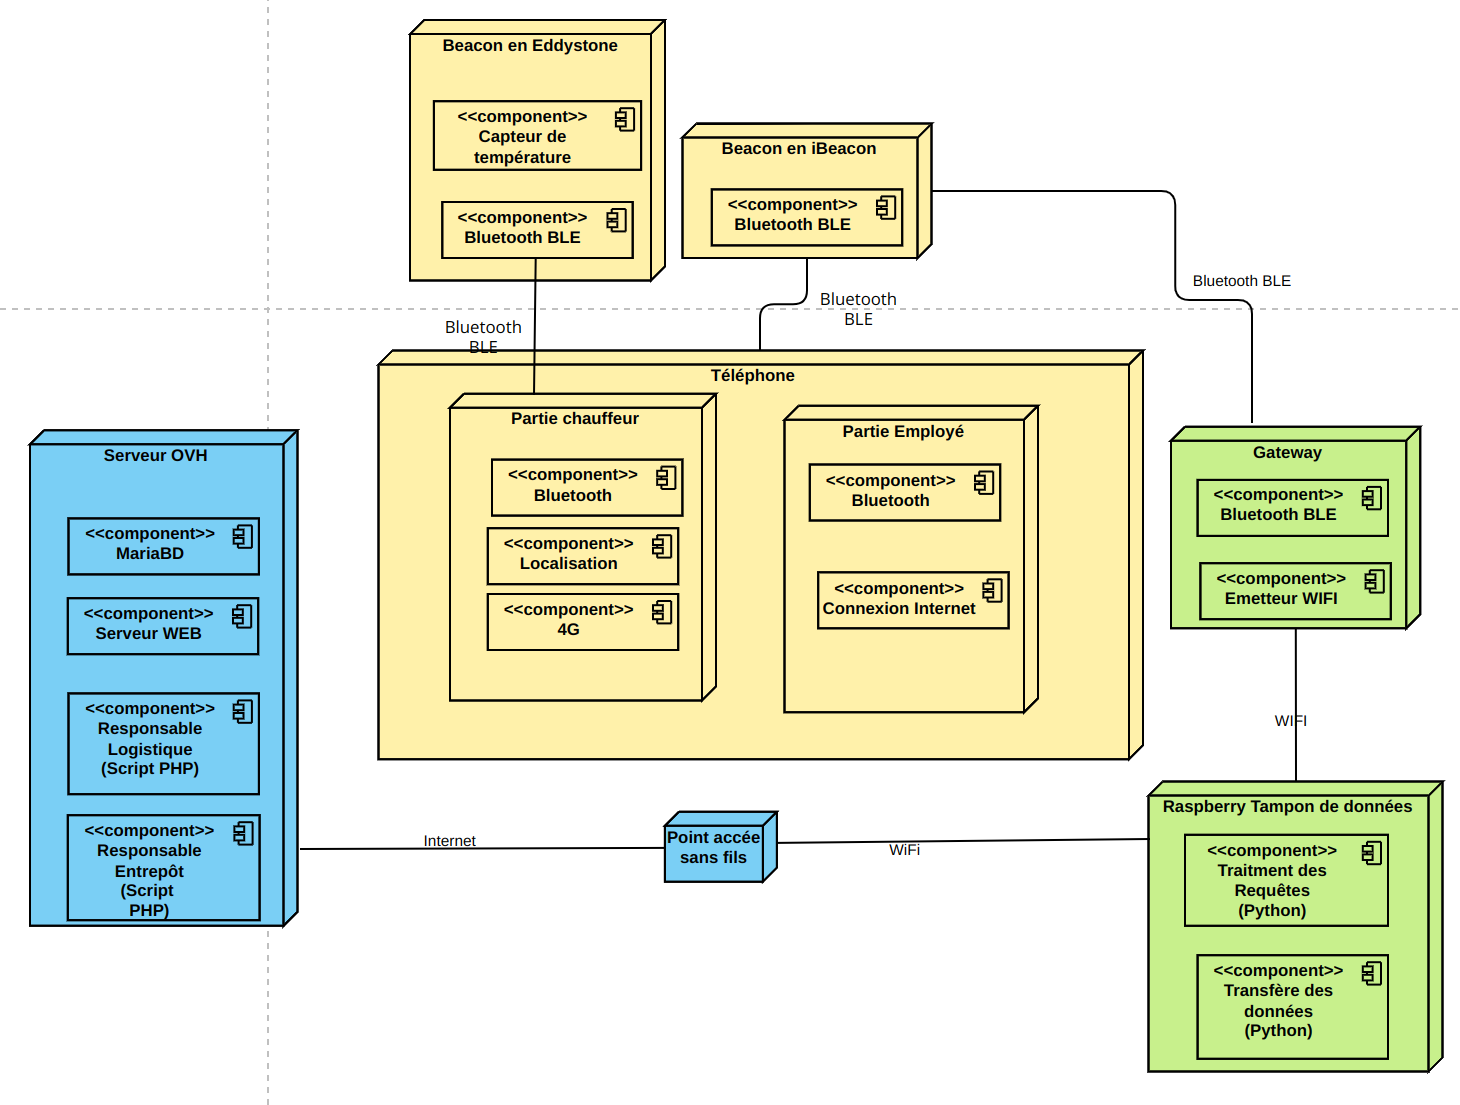
\includegraphics[scale=0.14]{Images/diagramme_deploiement.png}
        \caption{}
        \label{diagramme_deploiement}
    \end{subfigure}
    \begin{subfigure}[b]{0.45\textwidth}
        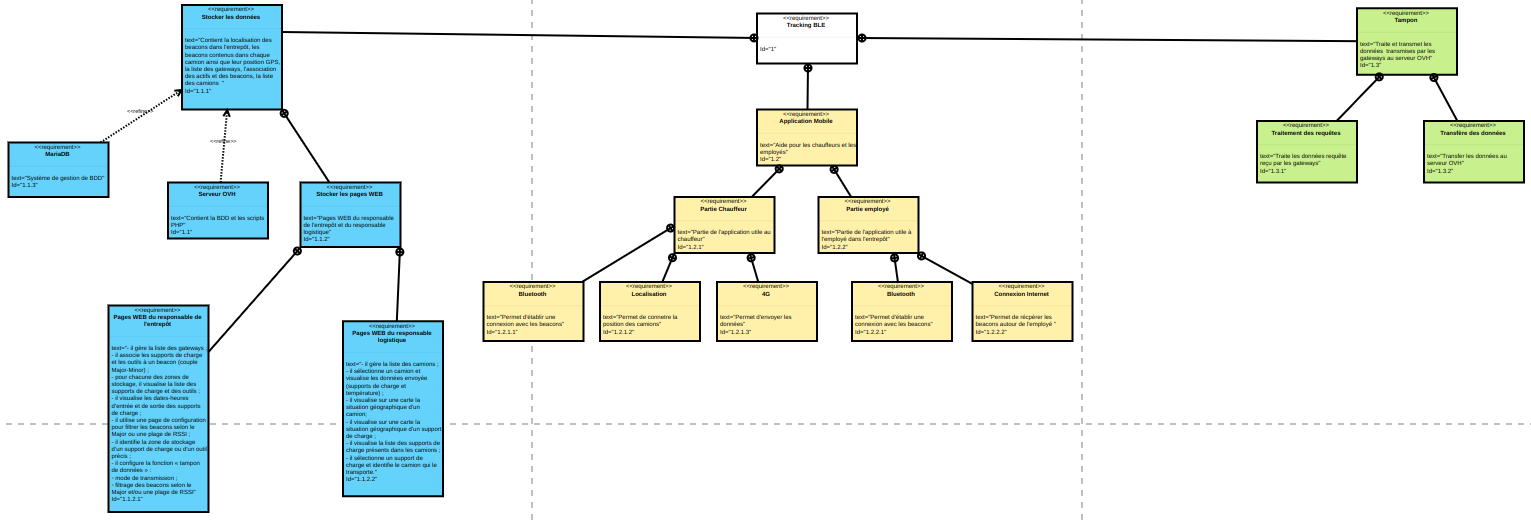
\includegraphics[scale=0.14]{Images/diagramme_exigence1.png}
        \caption{}
        \label{diagramme_exigences1}
    \end{subfigure}
    \caption{}
\end{figure}

\begin{figure}[h!]
    \centering
    \begin{subfigure}[b]{0.45\textwidth}
        \centering
        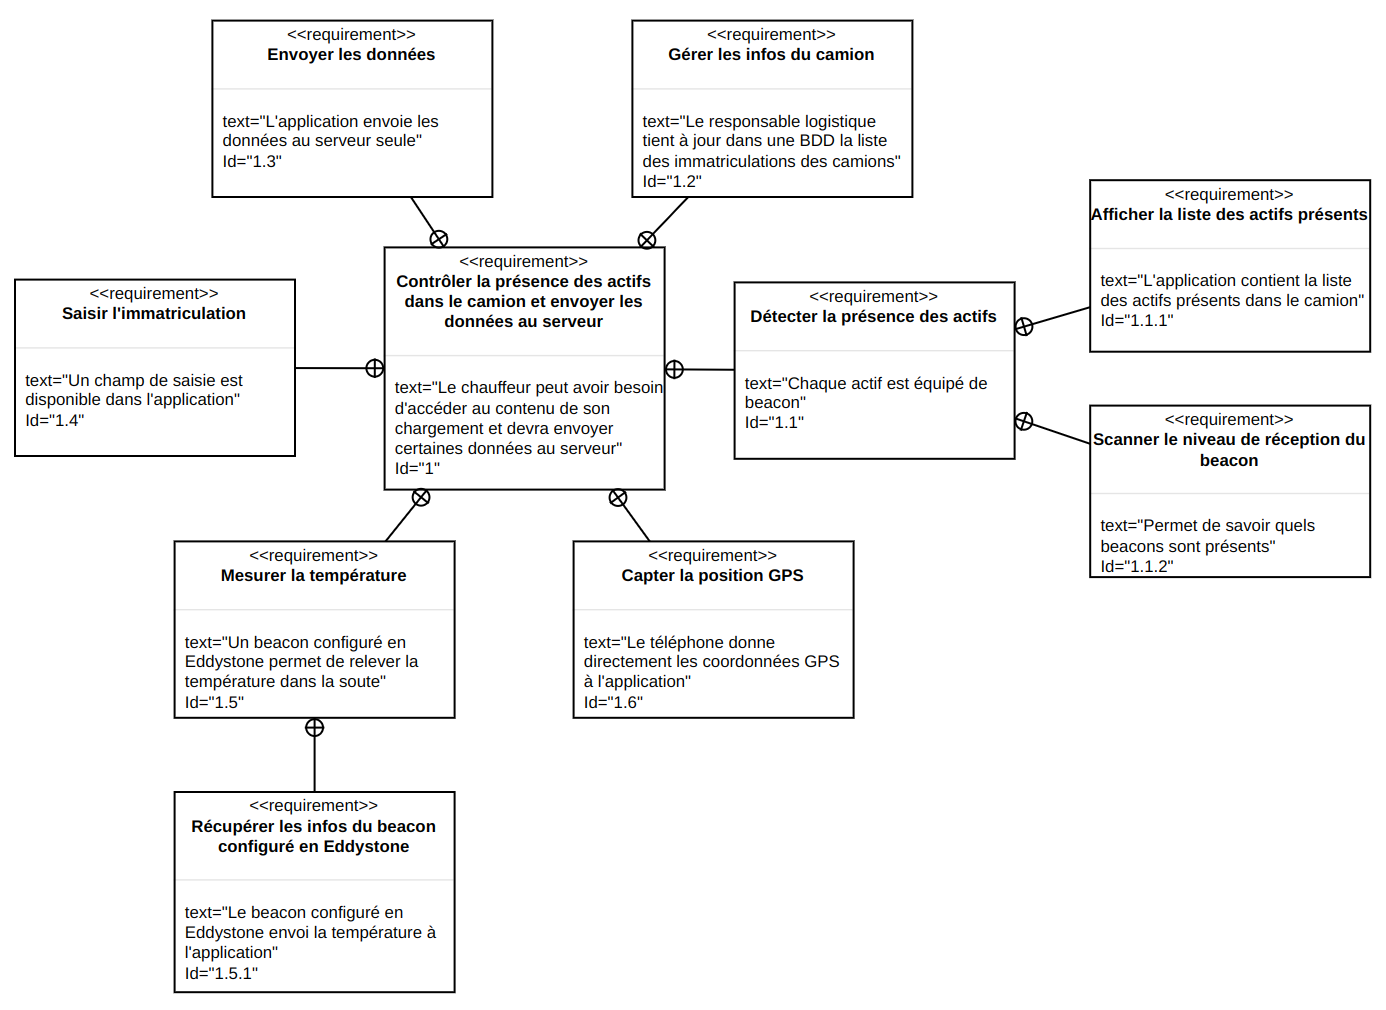
\includegraphics[scale=0.14]{Images/diagramme_exigences_camion.png}
        \caption{}
        \label{diagramme_exigences_camion} 
    \end{subfigure}
    \begin{subfigure}[b]{0.45\textwidth}
        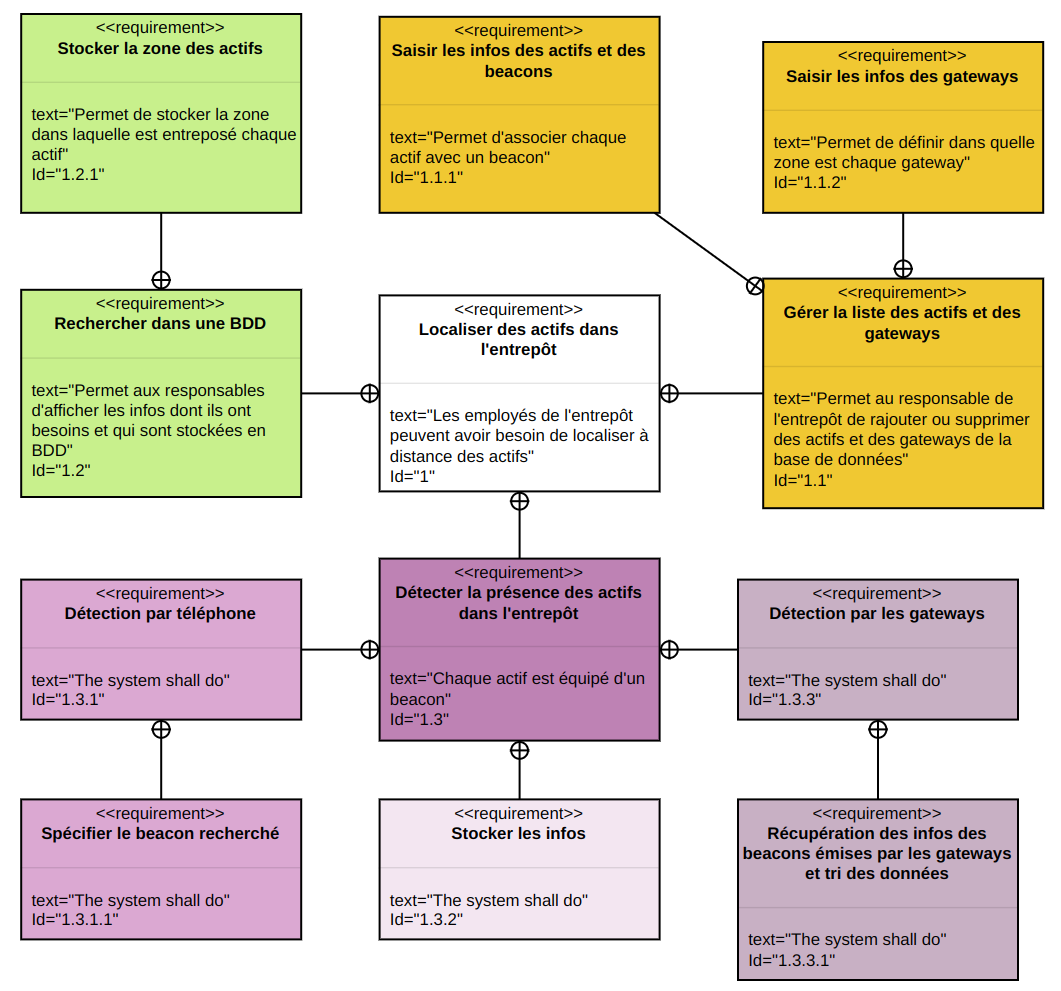
\includegraphics[scale=0.14]{Images/diagramme_exigences_entrepot.png}
        \caption{}
        \label{diagramme_exigences_entrepot}
    \end{subfigure}
    \caption{}
\end{figure}

\begin{figure}[h!]
    \centering
    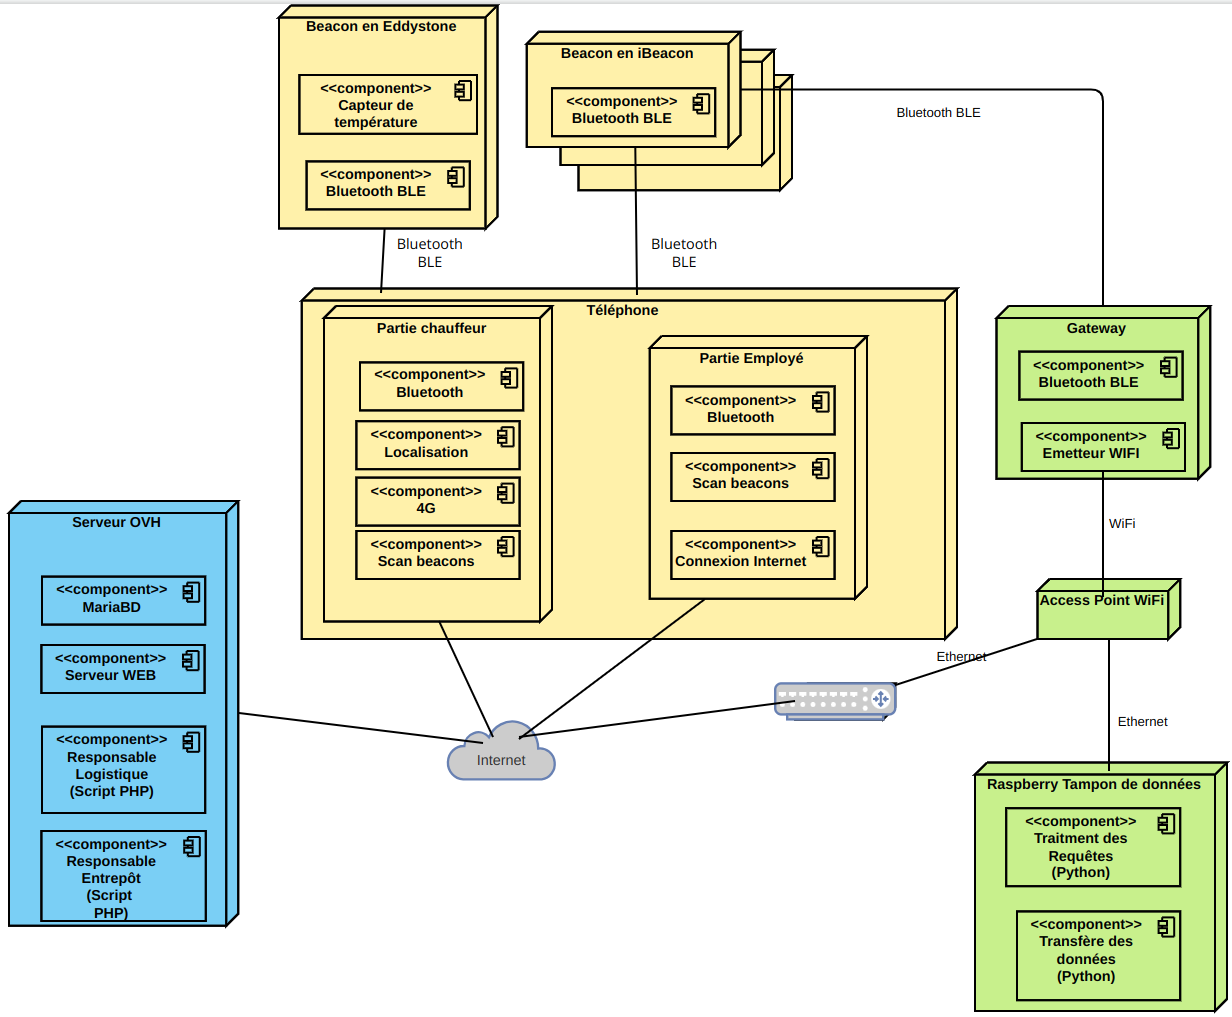
\includegraphics[scale=0.2]{Images/diagramme_deploiement2.png}
    \caption{}
    \label{diagramme_deploiement2}
\end{figure}

\begin{figure}[h!]
    \centering
    \begin{subfigure}[b]{0.45\textwidth}
        \centering
        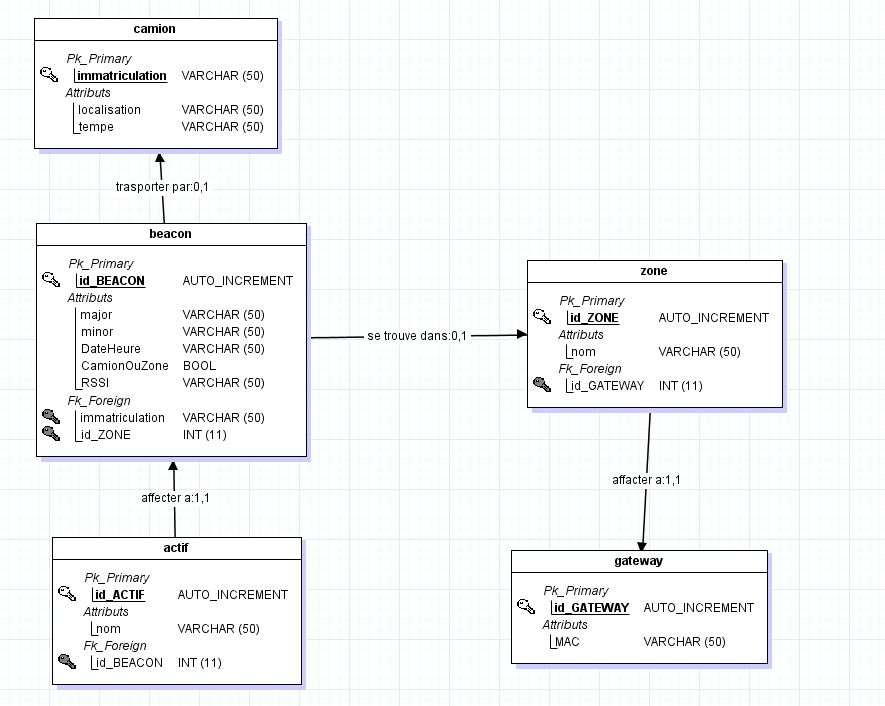
\includegraphics[scale=0.14]{Images/MLD_proposition_nous.png}
        \caption{}
        \label{MLD_proposition_nous} 
    \end{subfigure}
    \begin{subfigure}[b]{0.45\textwidth}
        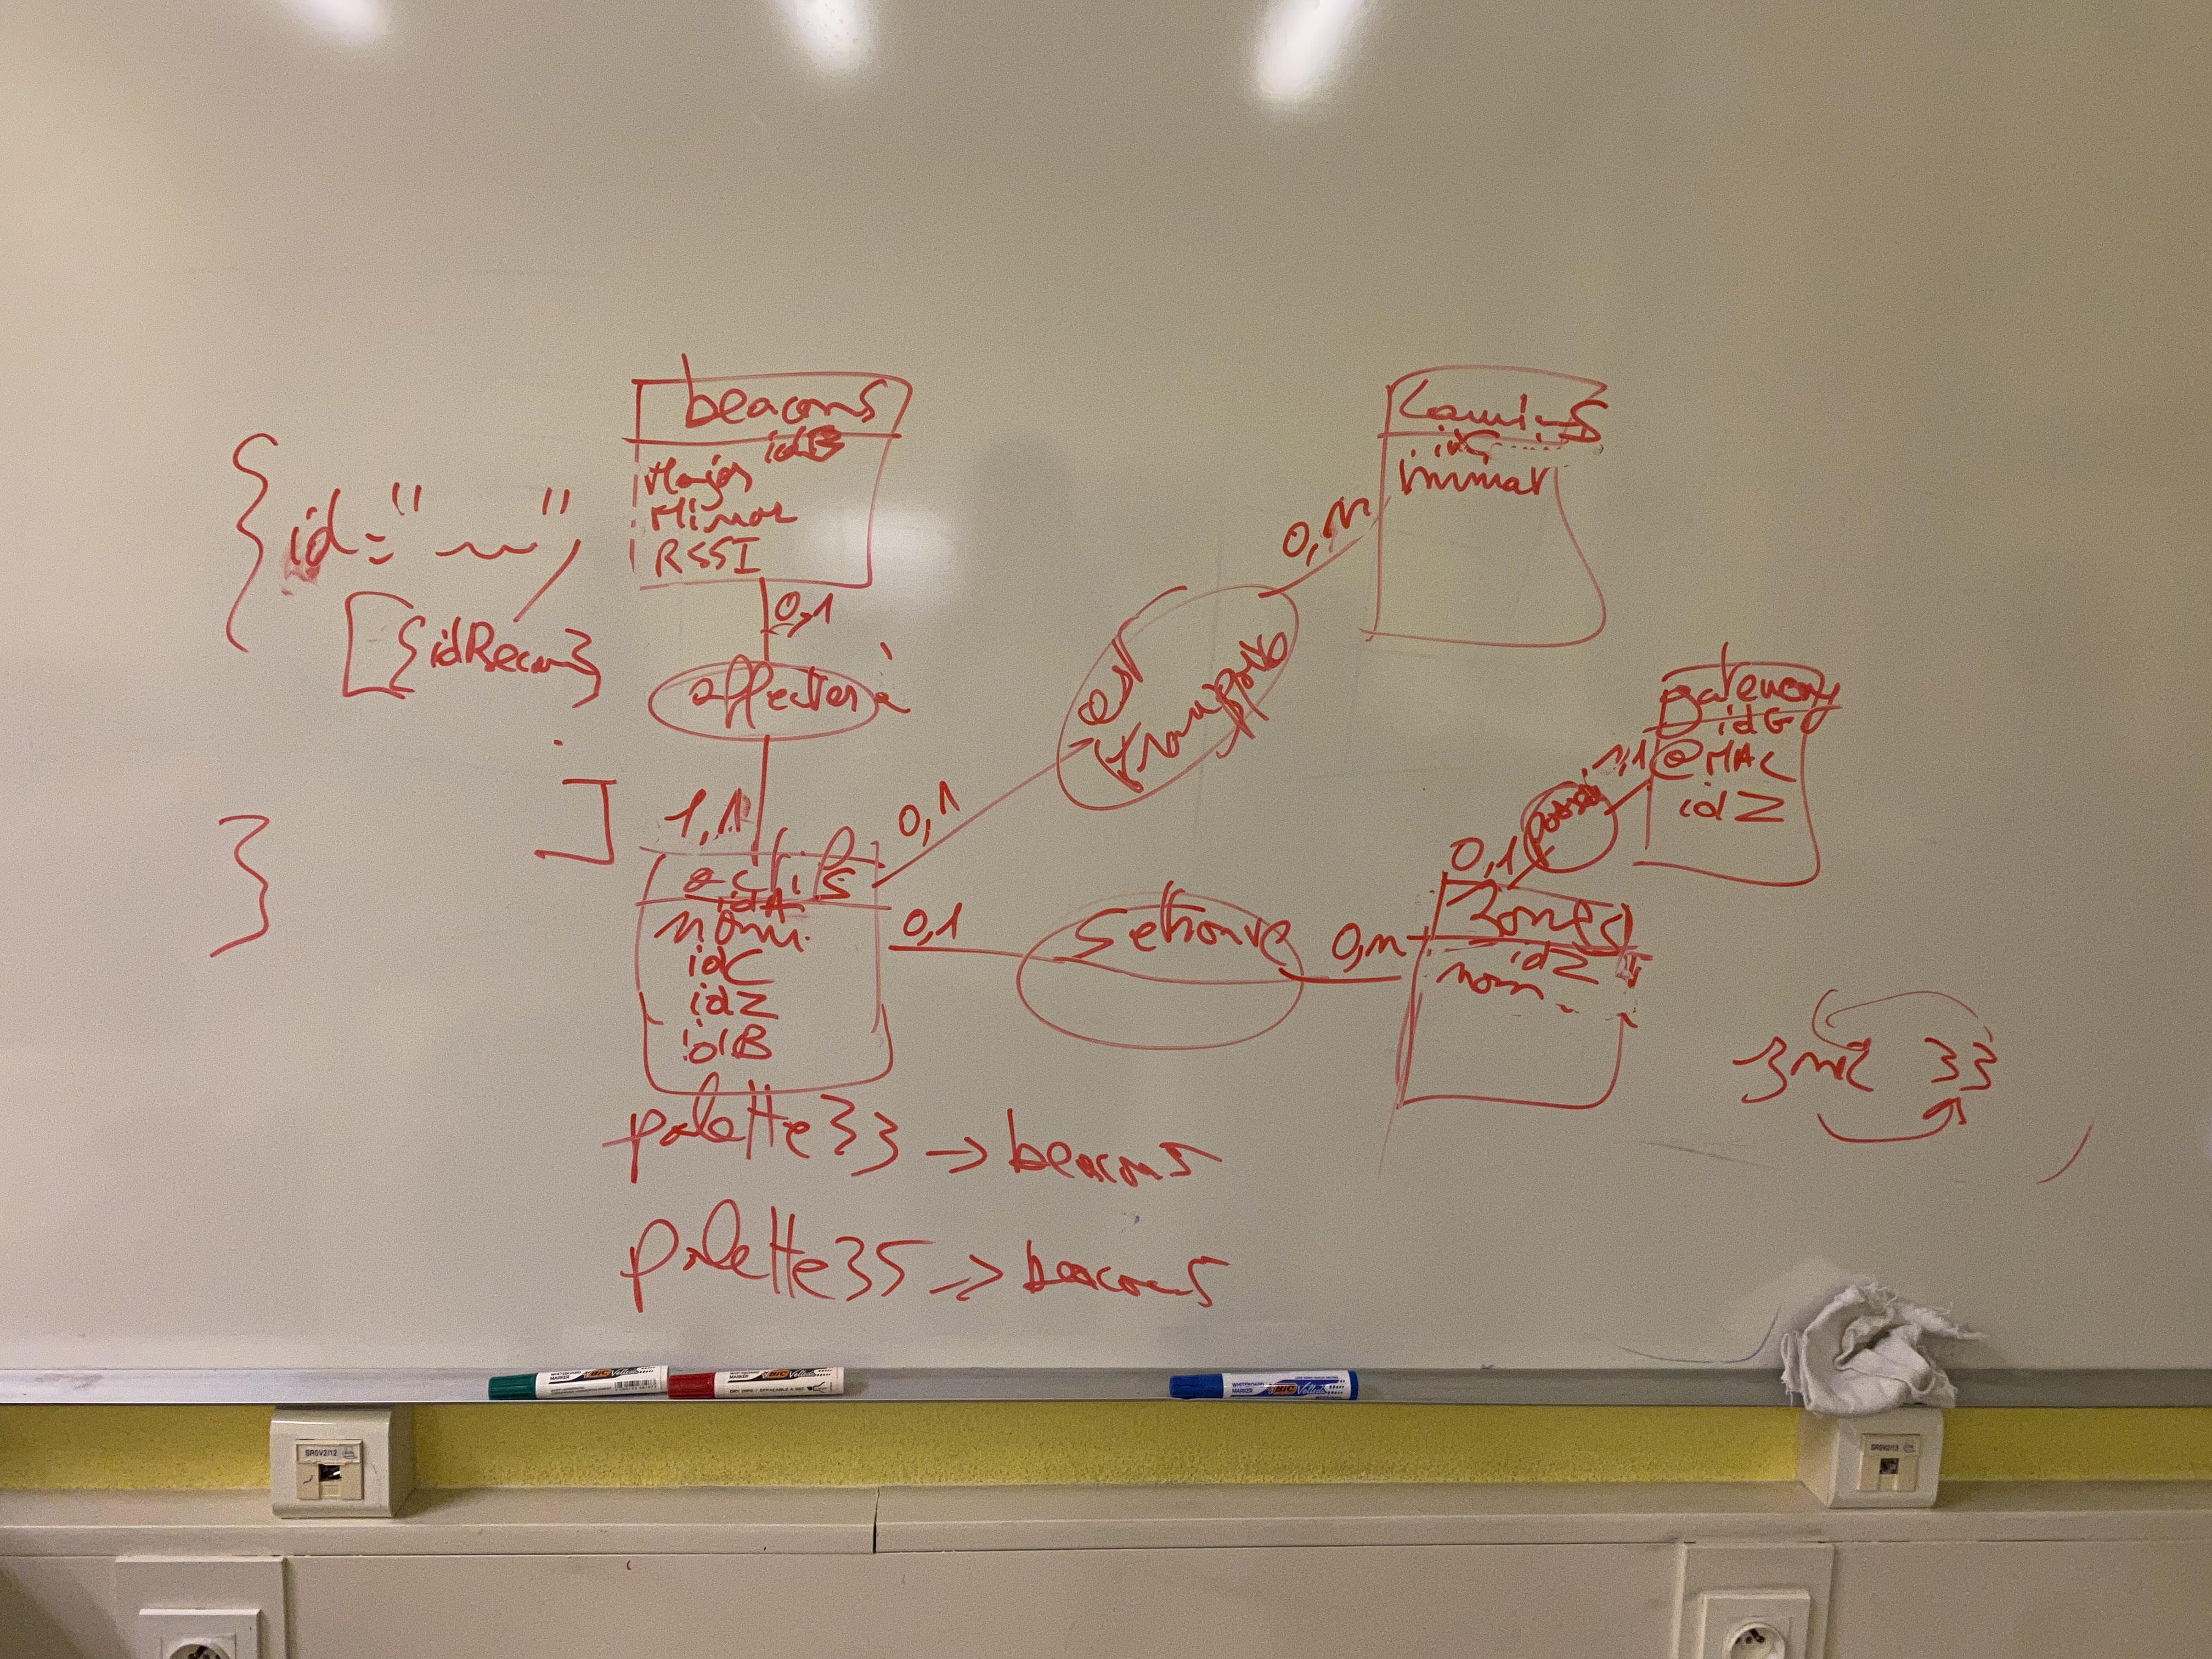
\includegraphics[scale=0.14]{Images/MLD_proposition_hacquard.jpg}
        \caption{}
        \label{MLD_proposition_hacquard}
    \end{subfigure}
    \caption{}
\end{figure}

\begin{figure}[h!]
    \centering
    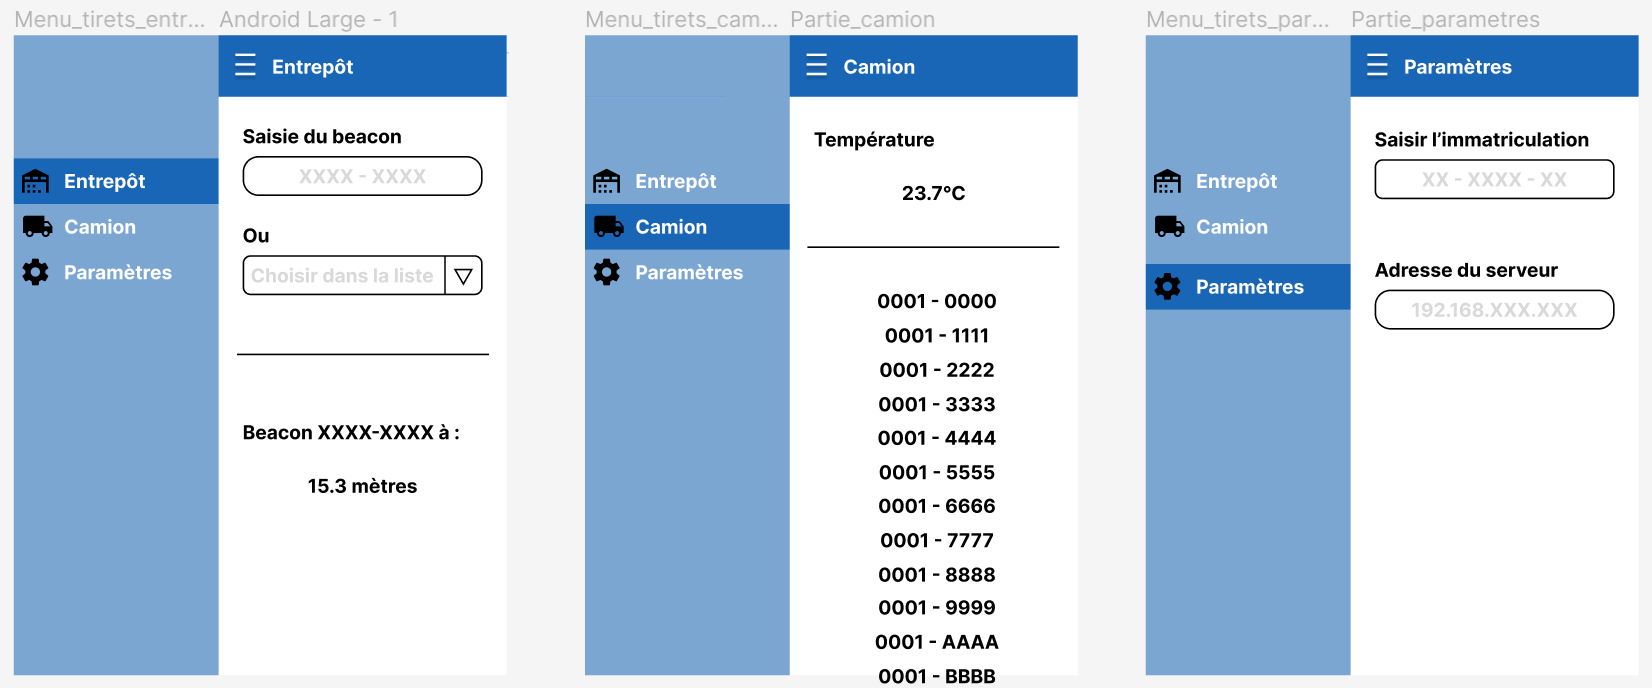
\includegraphics[scale=0.2]{Images/figma_v1.png}
    \caption{}
    \label{figma_v1}
\end{figure}

\end{document}
